% -*- root: main.tex -*-
% @Author: Oscar Esteban
% @Date:   2015-07-23 12:42:56
% @Last Modified by:   Oscar Esteban
% @Last Modified time: 2015-07-23 12:52:01

\documentclass[tikz]{standalone}
\usepackage{graphicx}

\usepackage[T1]{fontenc}
\usepackage{charter}

\begin{document}
\begin{tikzpicture}
  \node[](fig01a) at (0,11.8)
    {\hspace*{20pt}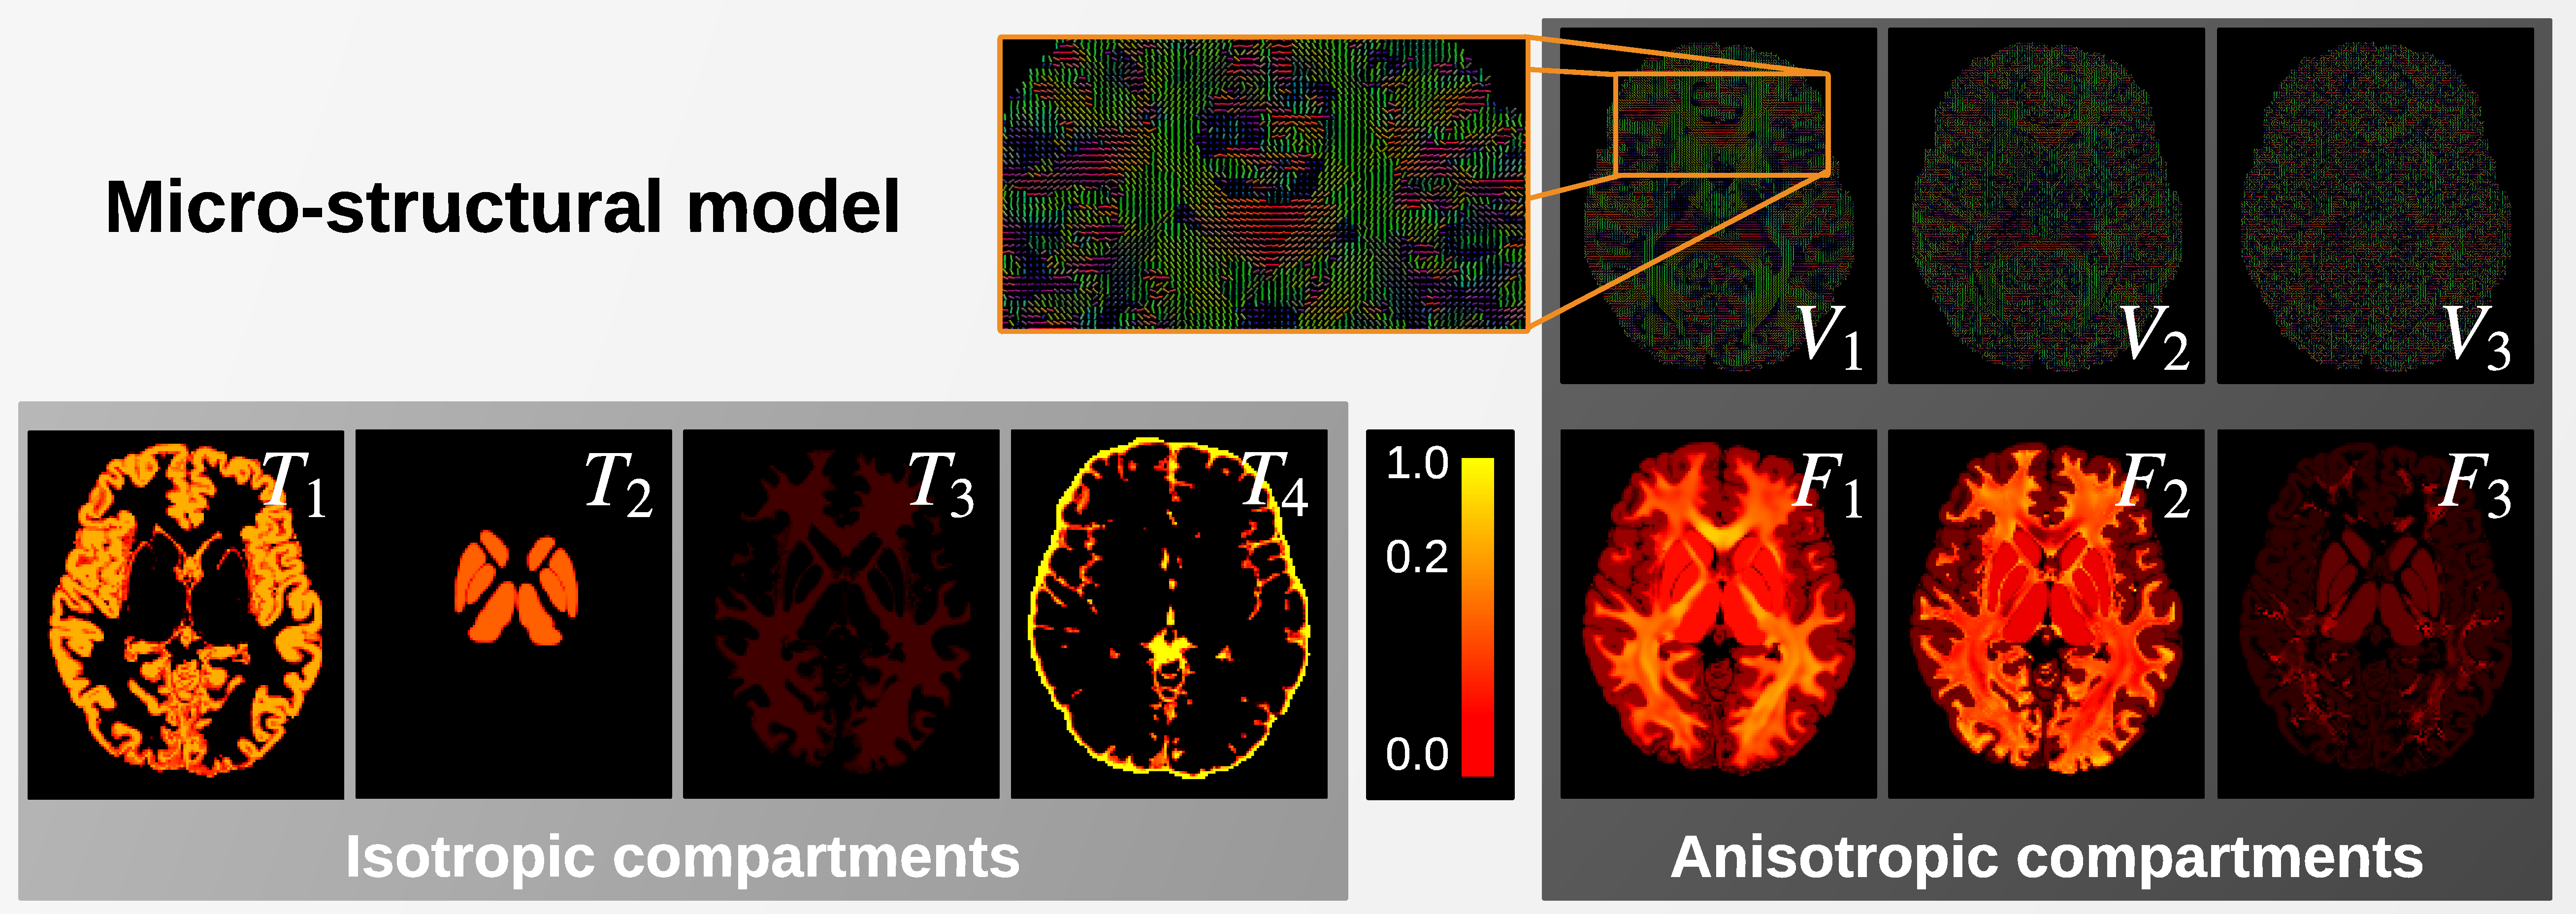
\includegraphics[width=21cm]{figures/figure01A}};
  \node[](fig01b) at (0,0)
    {\hspace*{20pt}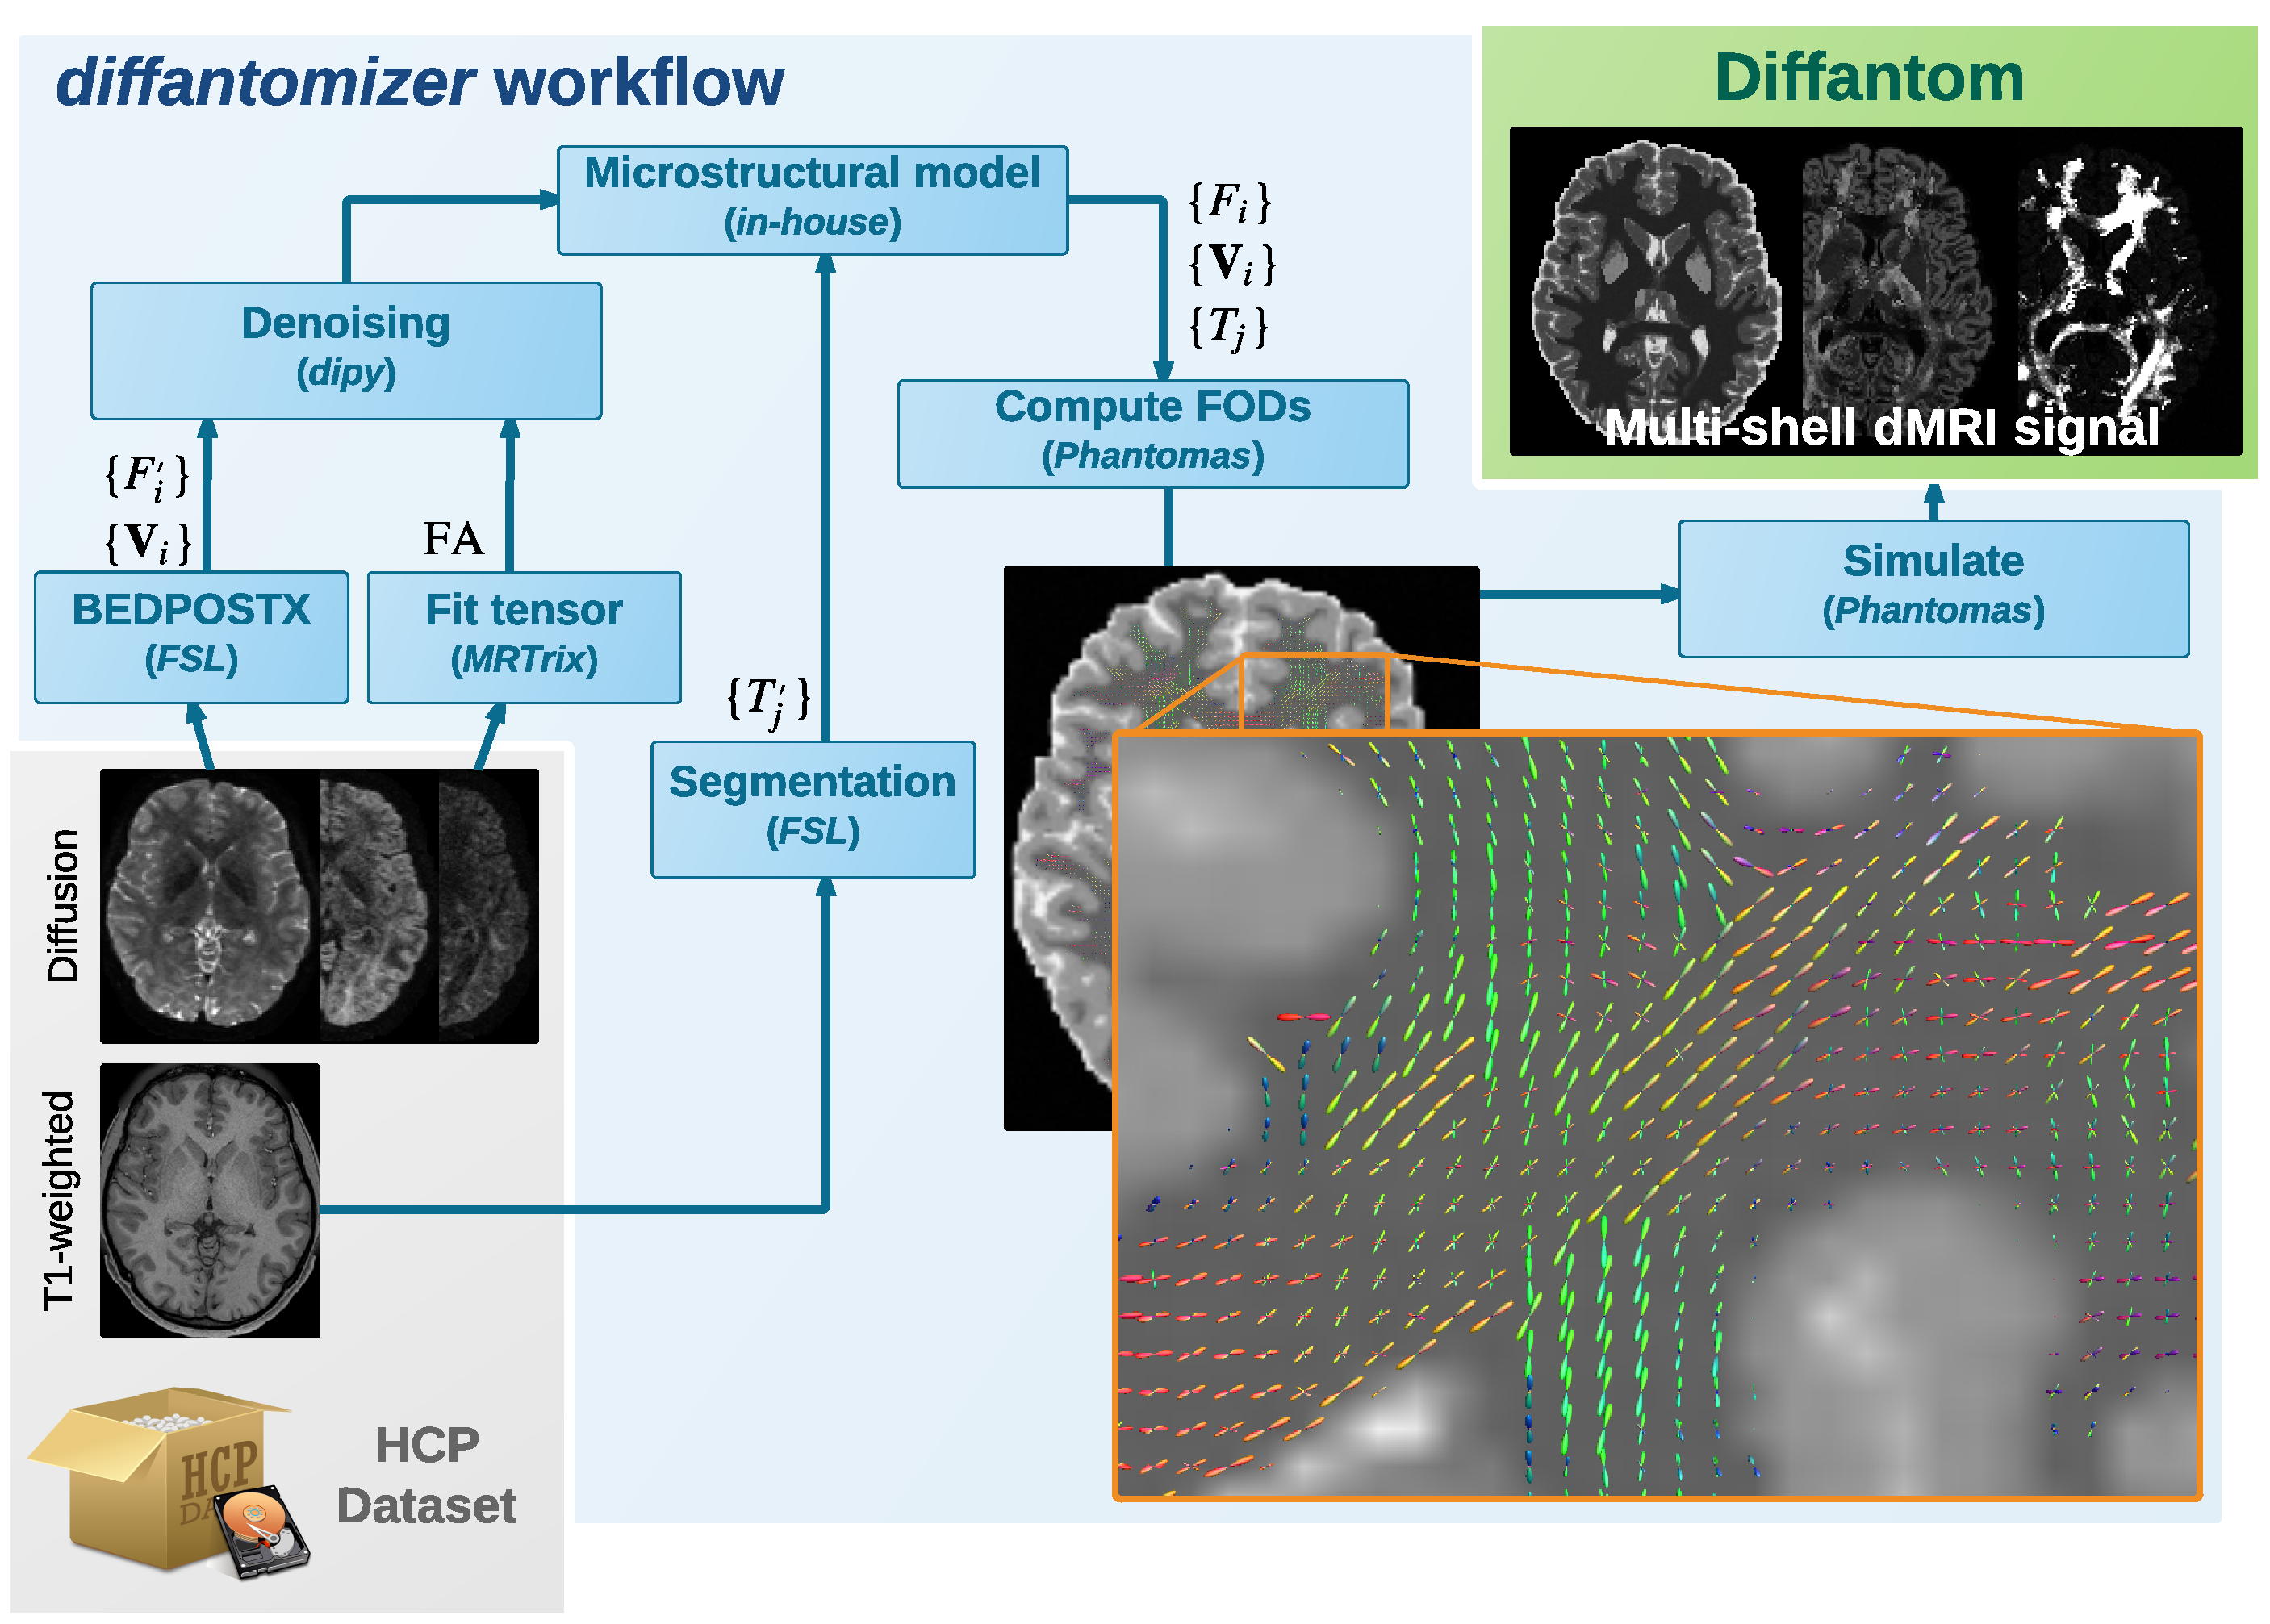
\includegraphics[width=21cm]{figures/figure01B}};
  \node[circle, text=black] at (-10.7,15.0) {\Huge \textbf{A}};
  \node[circle, text=black] at (-10.7,6.55) {\Huge \textbf{B}};
\end{tikzpicture}
\end{document}